\chapter{Der Client}
Dieses Kapitel beschäftigt sich mit dem Smartphone Client, der den Projektnamen AmbientClient trägt. Hierbei wird auf die Konzipierung des Clients sowie den Ablauf einer anzulegenden Umgebung und das Senden dieser eingegangen. 

\section{Konzipierung und Entwicklung der Benutzeroberfläche}
Nach der Festlegung der Lösungsstrategie, die InstantAmbient verfolg, musste ein Bedienkonzept für die App erarbeitet werden. Diese soll, wie schon mehrfach angesprochen wurde, schnell verständlich und kurze Bedienwege für den Benutzer bereitstellen. \\ 
Wie im Kapitel der Konfigurationen bereits angesprochen gibt es Sektionen. Da InstantAmbient sowohl für Autos als auch für Hotels funktionieren soll, wurde eine Allgemeine Konfiguration die elementare Möglichkeiten enthält konstruiert. Da diese sozusagen als Globale Konfiguration dienen, werden sie mit dem Start der Anwendung abgefragt. Dies gibt den/der BenutzerIn die Möglichkeit von vornherein die ersten Einstellungen vorzunehmen und auf seinem Gerät zu speichern.  

\begin{figure}[H]
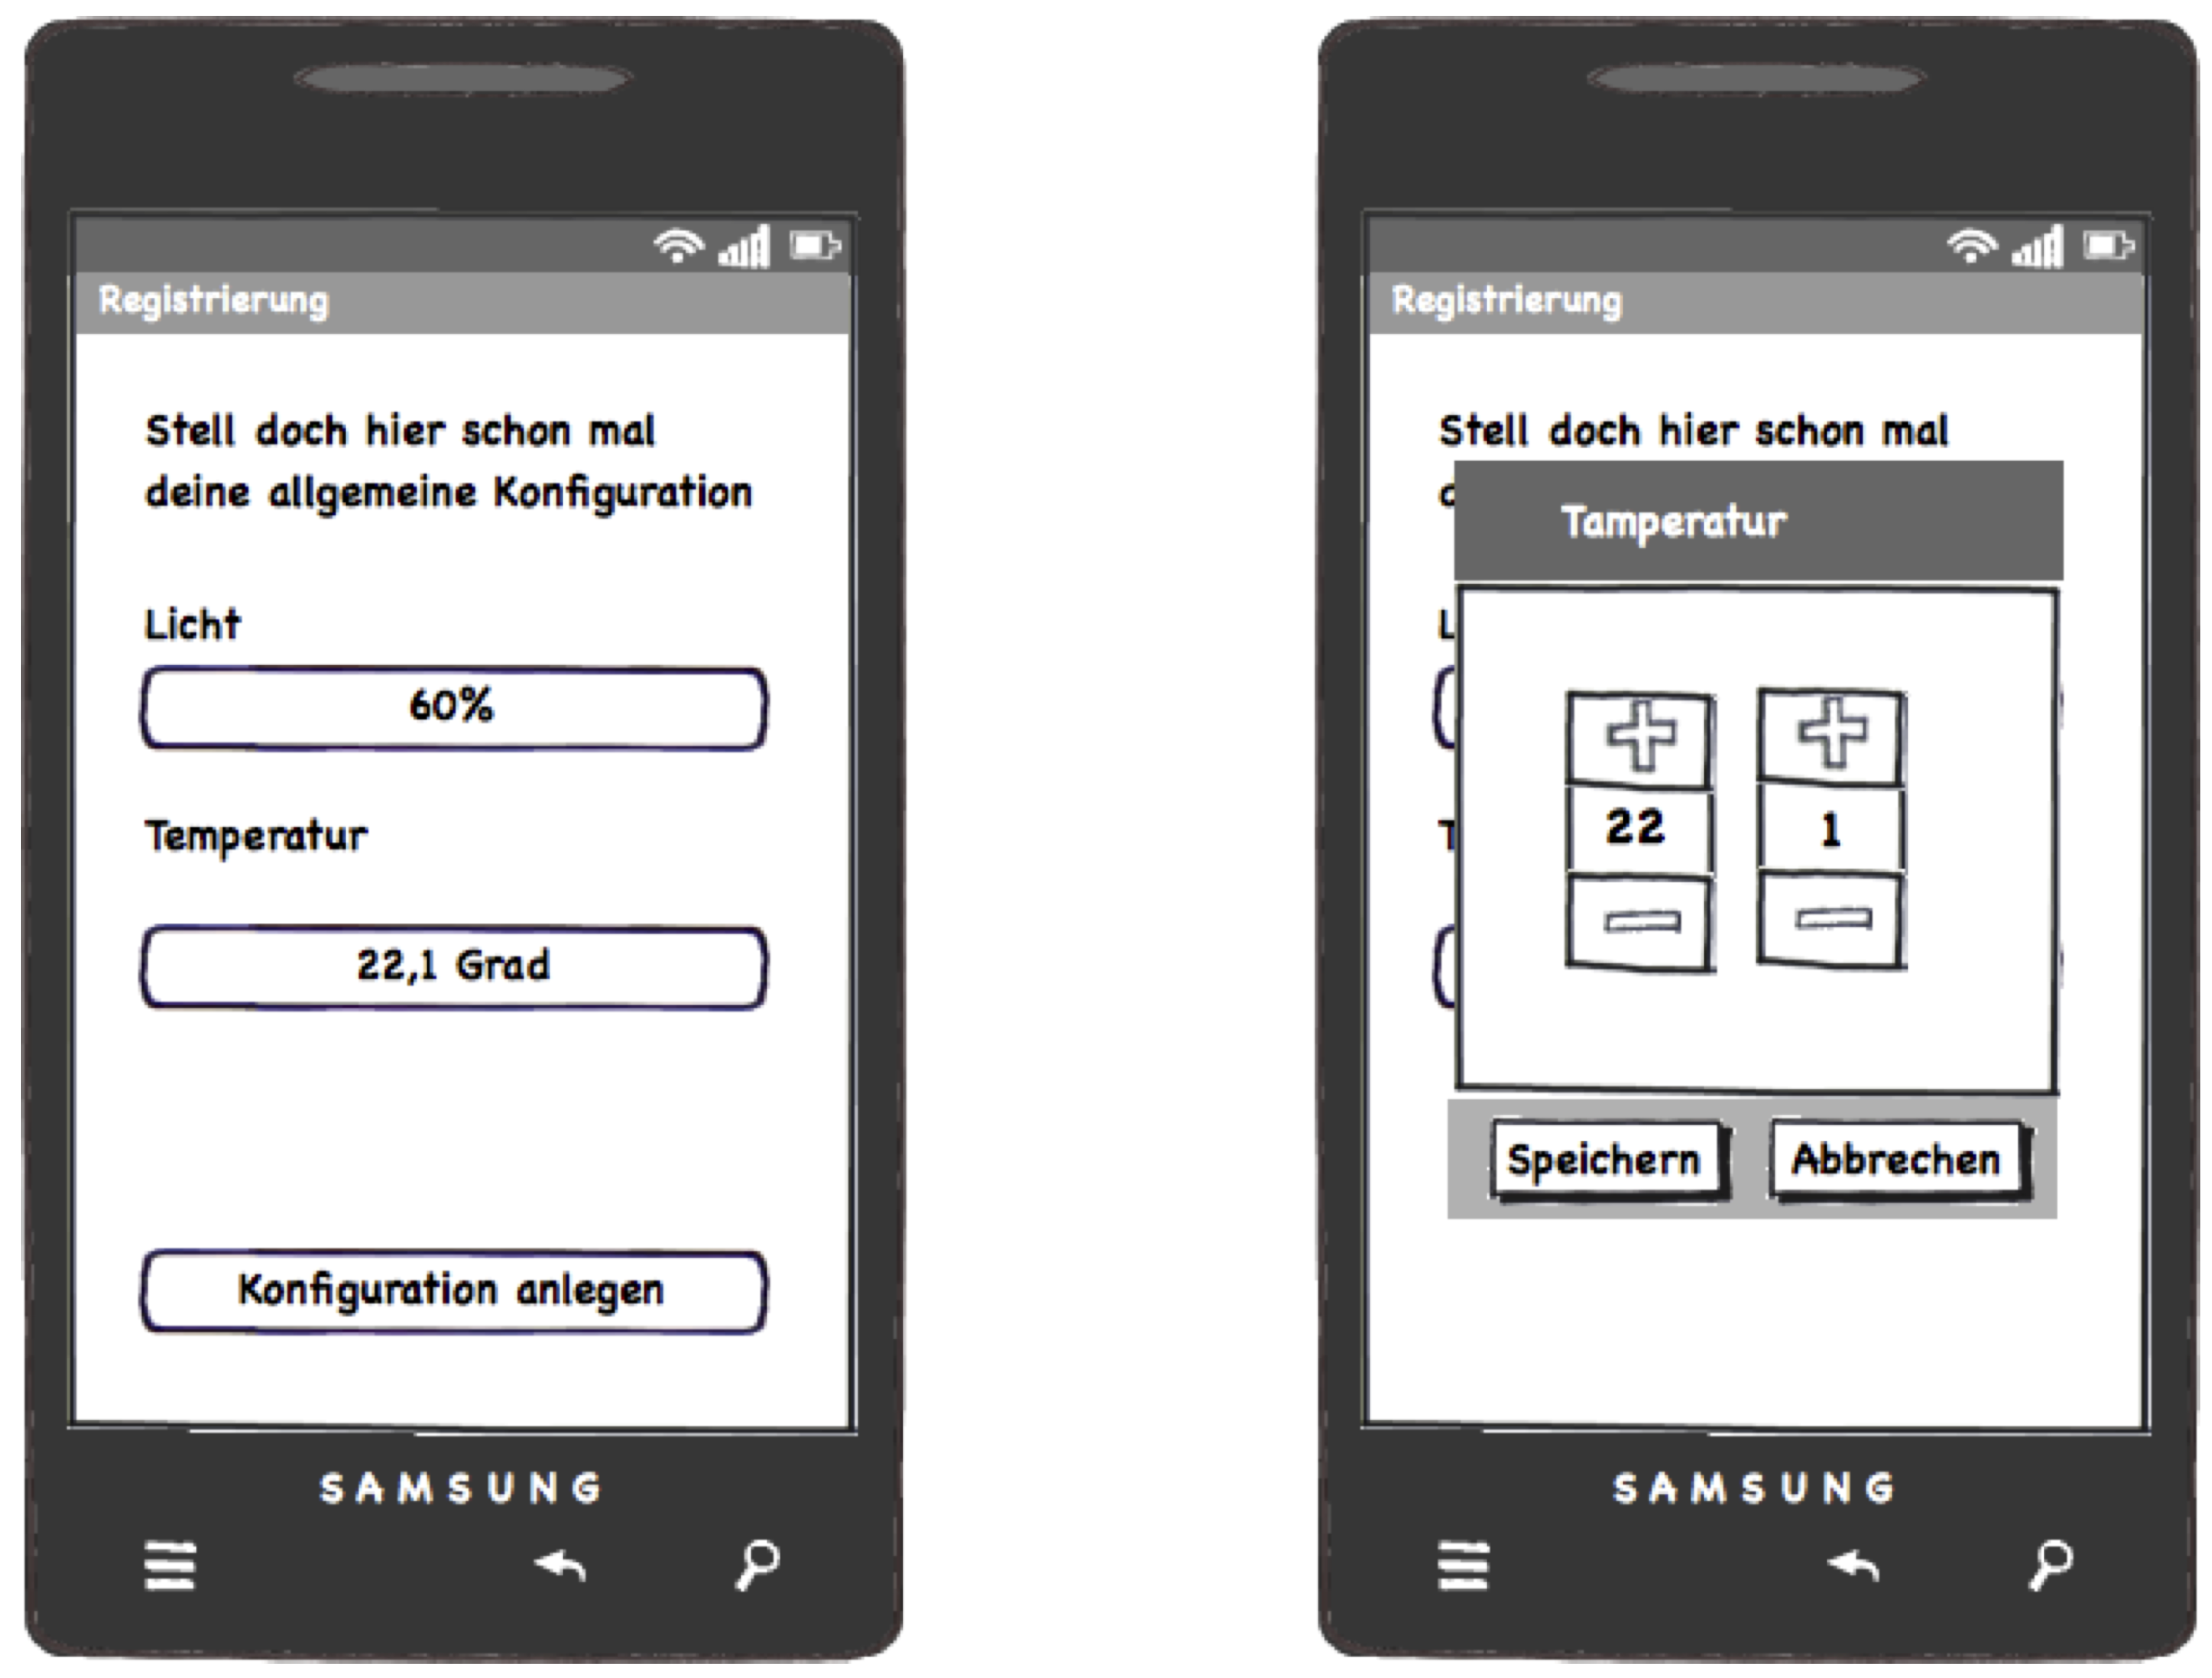
\includegraphics[width=12.5cm]{MockUps/Registrierung}
\caption{MockUp der Registrierung}
\end{figure}

Nachdem der/die BenutzerIn diese angelegt hat, wird er/sie in die Umgebungsübersicht geführt. Hier sieht er/sie alle von ihm/ihr angelegten Umgebungen. Durch das anklicken dieser kommt er/sie auf die Detailseite der Umgebung und kann diese gegebenenfalls ändern.       
Des Weiteren hat er/sie die Möglichkeit in der Übersicht im Menü eine neue Umgebung anzulegen oder die Allgemeine Konfiguration zu ändern. Dadurch ist diese von den Umgebungen getrennt veränderbar. Allerdings haben die Benutzer die Möglichkeit die Allgemeinen Konfigurationsdaten für eine Spezifische Umgebung zu ändern ohne die allgemeine Konfiguration zu verändern. 

\begin{figure}[H]
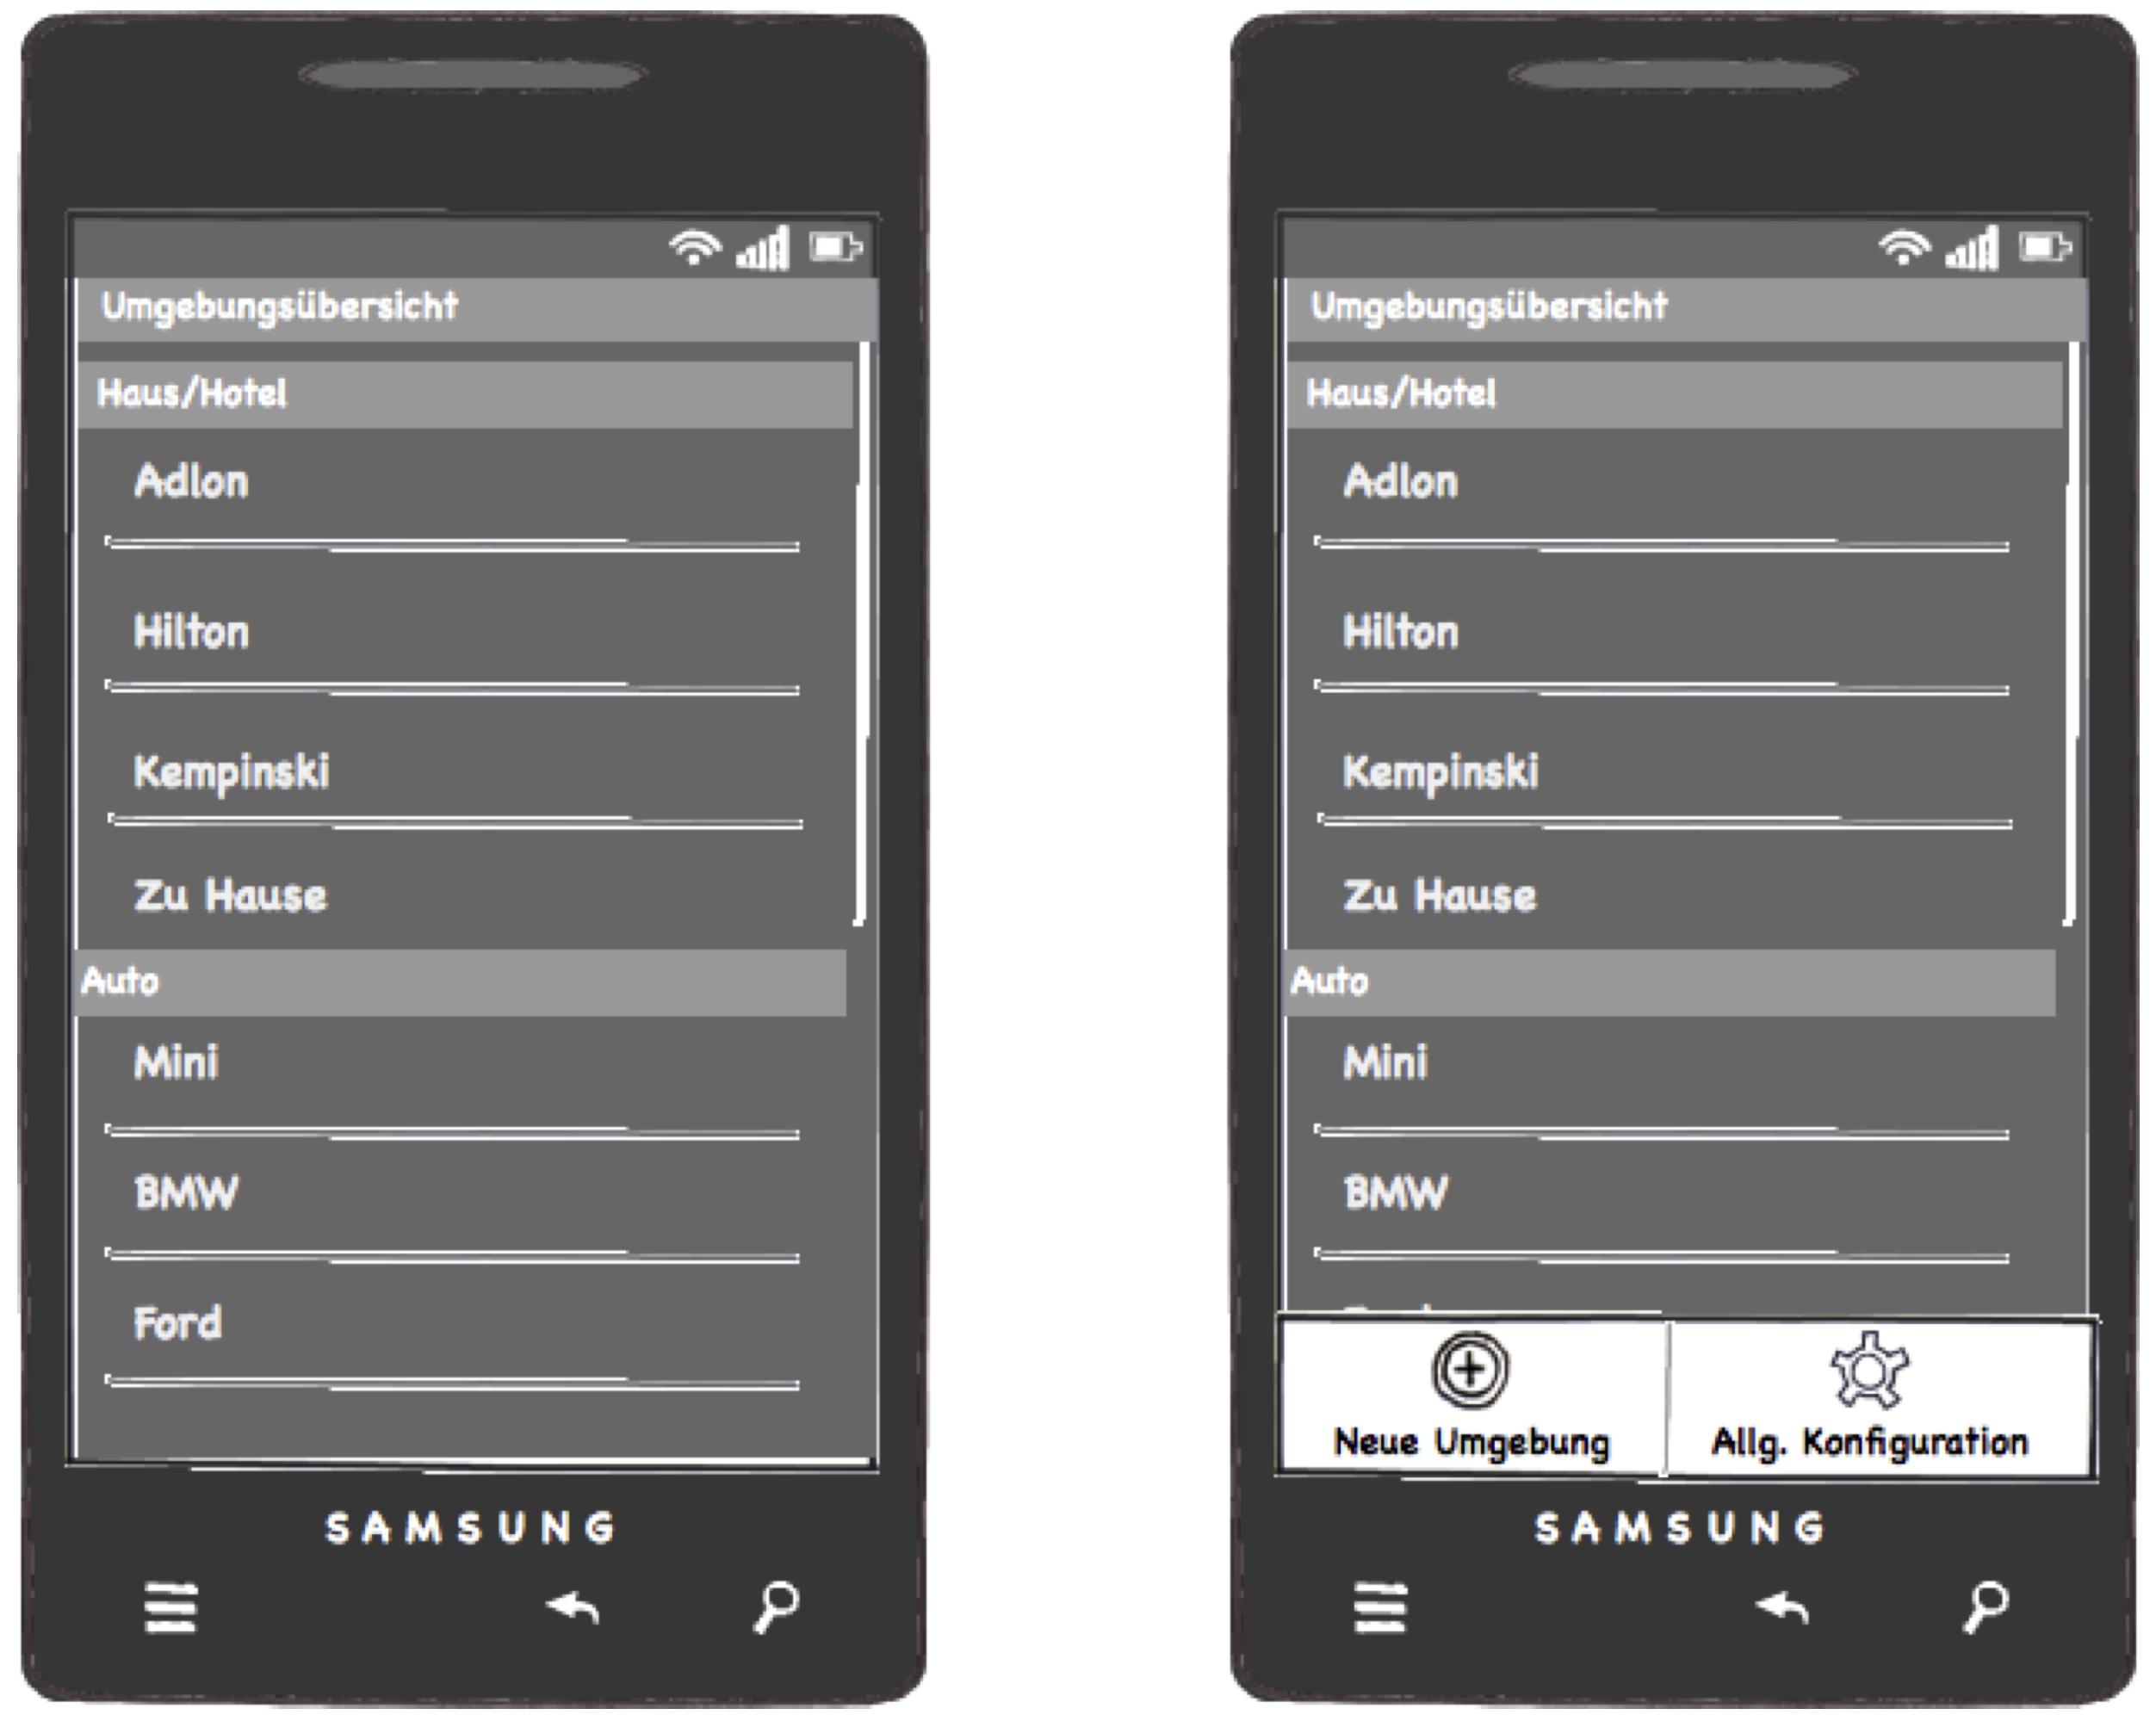
\includegraphics[width=12.5cm]{MockUps/Umgebung}
\caption{MockUp der Umgebungsübersicht}
\end{figure}

Es gibt also drei verschiedene Hauptansichten. Die Umgebungsübersicht, die Umgebungsansicht und die Ansicht für die Allgemeine Konfiguration. Die Anwendung wurde sehr schlicht gehalten und nicht mit Auffälligen optischen Spielereien bestückt. Die Oberfläche soll die Benutzer nicht ablenken, sondern den Fokus auf die Einstellungen legen. 
\\\\
Des Weiteren wurde auch eine mögliche Konzeption entwickelt wenn sich ein/e BenutzerIn zum zweiten mal in einem Hotel befindet, nur das dieses mal die Ausstattung des Zimmers mehr Möglichkeiten bietet. Hierbei sollte das Backend den Client über die neuen Möglichkeiten informieren und dieser meldet dies dem/der BenutzerIn und gibt ihm/ihr hierbei gleich die Möglichkeit ein neues Profil für die Umgebung anzulegen. Dieses Konzept ist aber nicht in der Anwendung umgesetzt worden. Da hierbei das Ziel war eine einfache Konfiguration zu erstellen und zu Übertragen.

\begin{figure}[H]
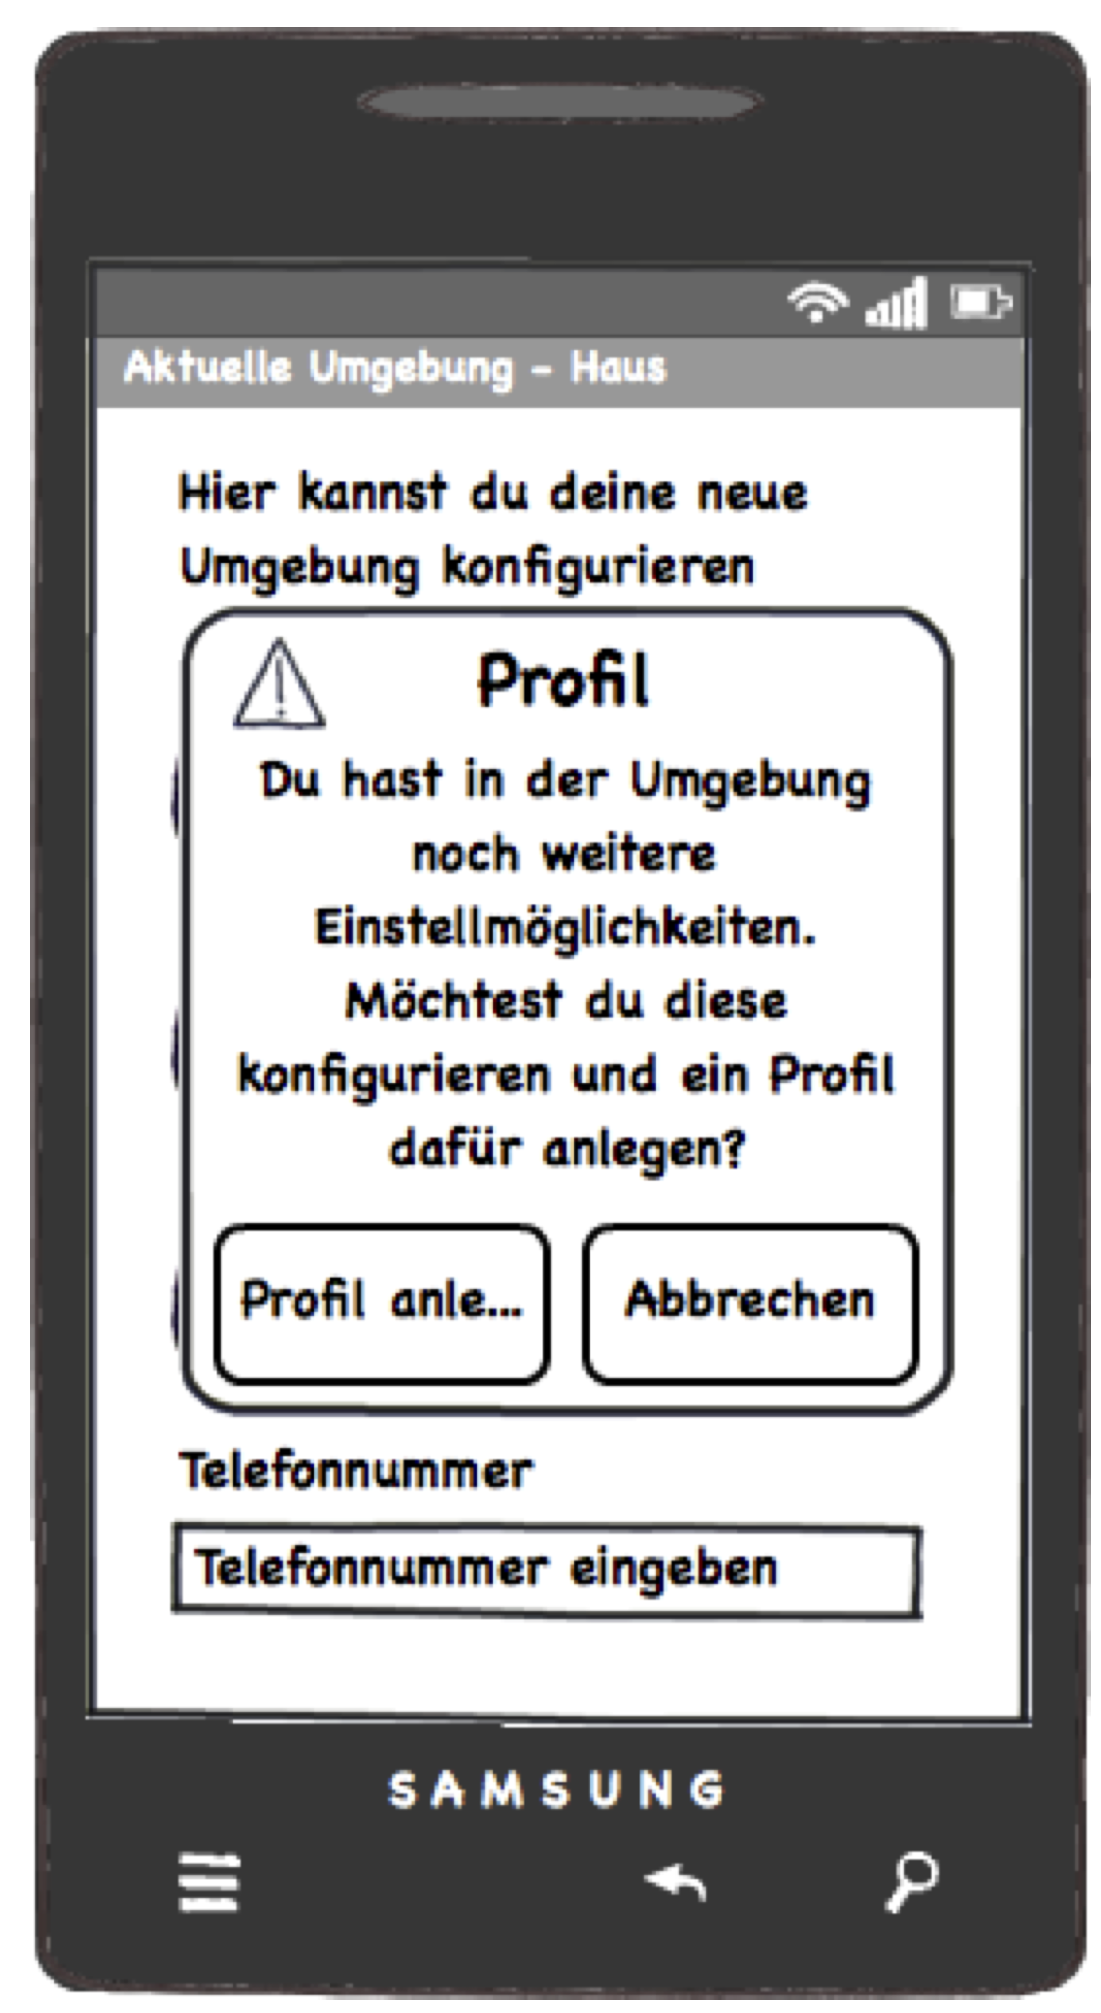
\includegraphics[width=6cm]{MockUps/Erweiterung}
\caption{MockUp der Profilerweiterung}
\end{figure}

\section{Umsetzung} 
Nach dem die Konzeption und die Benutzerführung anhand der Mock-Ups stand, wurde die Anwendung entwickelt. Bei der Verwendung des SDK wurde auf die letzte verbreitete Smartphone Version von Android zurückgegriefen. Damit die Konfiguration vom Licht oder von der Temperatur eingestellt werden kann wurde ein NumberPicker verwendet. Dies führte ein Problem mit sich, auf das im Abschnitt Probleme eingegangen wird. Als Datenbank wurde die von Android bereitgestellte SQLite Datenbank verwendet. Ein wichtiger Bestandteil neben der Oberfläche ist die Bluetoothschnittstelle. \\
Diese wurde als Service implementiert und kann somit unabhängig von der Anwendung im Hintergrund laufen. Dies ist ein wichtiger Punkt vom AmbientClient, da der Benutzer möglichst wenig mit dem starten des Übertragungablauf zu tun haben soll. Zumindest soll es für den Benutzer nicht offensichtlich sein. In dem Prototypen wird der Service mit dem öffnen der Anwendung, in der Umgebungsübersicht gestartet. Damit die Anwendung Bluetooth verwenden kann muss dieses zu aller erst eingeschalten werden. Dies wird beim Ersten Start, nachdem die Allgemeine Konfiguration angelegt wurde, abgefragt und der Benutzer wird gegebenenfalls darum gebeten dieses einzuschalten. Der Service kann jederzeit erweitern und verändert werden. Dies ist ein Grund warum diese Schnittstelle als Service aufgebaut wurde. Hierbei muss dieser aber den Namen der Einheit kennen mit der er sich verbinden soll, bevor er mit diesem ein Pairing durchführen kann. Sobald der Client etwas gefunden hat beginnt er eine Verbindung aufzubauen, die Daten aus der Datenbank zu laden und als JSON Objekt an den Connector zu senden. Da dies völlig automatisch im Hintergrund passiert, erhält der Benutzer keine Rückmeldung falls die Übertragung erfolgreich war.

\section{Probleme}

Ein Problem was sich bei Android als immer wiederkehrend zeigt ist, dass bei der Konzeption von Android einige Fehler gemacht wurden. Zum Beispiel ist es möglich den in der Anwendung verwendete NumberPicker in der Grafischen Oberfläche einzubauen, doch kann man diesen nicht im Code einbinden, da er erst ab dem API Level 11, welches auch als Android 3.0 bezeichnet wird, zur offenen Verfügung steht. Diese Android Version ist allerdings nur für Tablets. Aus diesem Grund mussten extra zwei Klassen die den NumberPicker bilden eingebunden werden. Es ist ein typisches Androidphänomen, dass gewisse Möglichkeiten erst in späteren Versionen bereitgestellt werden, obwohl der Ansatz schon seit API Level eins vorhanden ist. Ein weiteres Problem bei Android sind die verschiedenen Benutzeranischten. Jede Anwendung verfolgt ihren eigenen Weg. Es entsteht keine Einheitliche Struktur. Der einzigen Struktur zur Navigation ist das Menü welches mittels Taste aufgerufen werden kann und die Zurücktaste, die einen gegebenenfalls in die letzte Ansicht zurückbringt oder die App schließt.  


\section{Zusammenfassung Client}

Dieser Abschnitt sollte einen überblick über das gewählte Konzept, die Benutzerführung sowie die für den Prototypen Umgesetzten Funktionen geben. Im nächsten Abschnitt folgt die Umsetzung des Backend.  


